\documentclass{article}

\usepackage{hyperref}
\usepackage{pgfplots}

\usepgfplotslibrary{
    colorbrewer,
    groupplots,
}

\pgfplotsset{
    compat=1.17,
    cycle list/Set1,
    cycle list name=Set1,
    height=0.4\linewidth,
    width=0.9\linewidth,
}

\begin{document}

Here, I'll show some more customized examples.
A lot of MWEs can be found at the \href{http://pgfplots.sourceforge.net/gallery.html}{PGFPlots gallery}.

\section{Custom Functions}
\begin{figure}[h]
    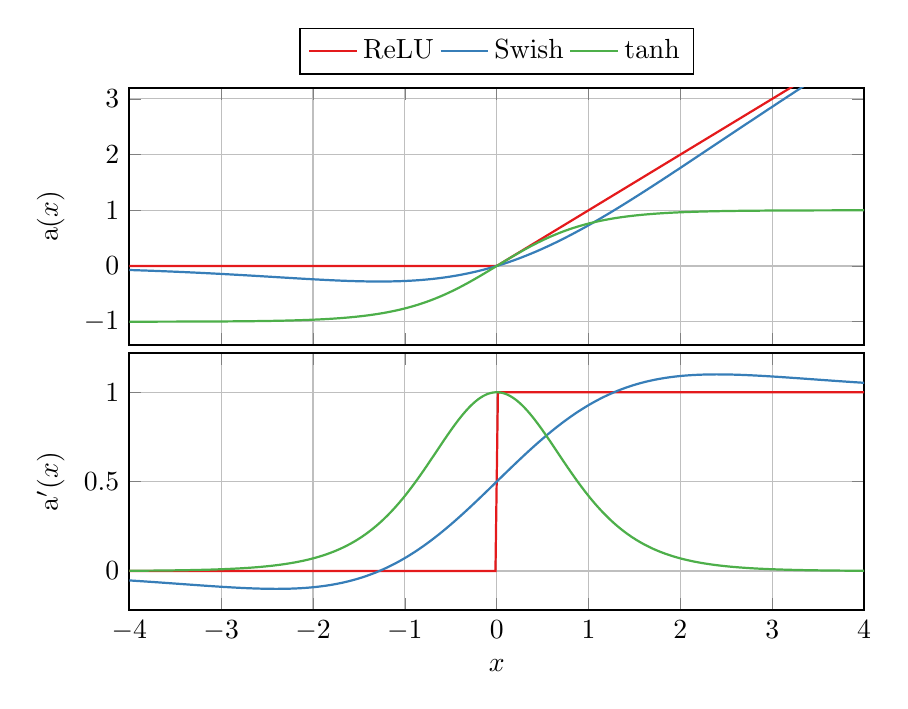
\begin{tikzpicture}[
            declare function={
                    relu(\x) = (\x > 0) * (\x);
                    d_relu(\x) = (\x > 0);
                    sigma(\x) = 1 / (1 + exp(-\x));
                    d_sigma(\x) = sigma(\x) * (1 - sigma(\x));
                    swish(\x) = \x * sigma(\x);
                    d_swish(\x) = sigma(\x) + \x * d_sigma(\x);
                    d_tanh(\x) = 1 - pow(tanh(\x), 2);
                },
        ]
        \begin{groupplot}[
                domain=-4:4,
                enlarge x limits=0,
                every axis/.append style={semithick},
                every axis plot/.append style={thick},
                grid=major,
                group style={
                        group size=1 by 2,
                        vertical sep=1mm,
                        xlabels at=edge bottom,
                        ylabels at=edge left,
                    },
                samples=300,
                xlabel={$x$},
            ]
            \nextgroupplot[
                legend style={
                        anchor=south,
                        at={(0.5,1.05)},
                        legend columns=5,
                    },
                xticklabels={,,},
                ylabel={$\mathrm{a}(x)$},
                ymax=3.2,
                ytick={-1, 0, ..., 3},
            ]
            \addplot+ {relu(x)}; \addlegendentry{ReLU}
            \addplot+ {swish(x)}; \addlegendentry{Swish}
            \addplot+ {tanh(x)}; \addlegendentry{tanh}
            \nextgroupplot[
                ylabel={$\mathrm{a}^\prime(x)$},
            ]
            \addplot+ {d_relu(x)};
            \addplot+ {d_swish(x)};
            \addplot+ {d_tanh(x)};
        \end{groupplot}
    \end{tikzpicture}
    \caption{
        ReLU, swish and tanh activation functions with their derivatives.
    }
\end{figure}

\newpage
\section{Bar Plots}
\begin{figure}[h]
    \centering
    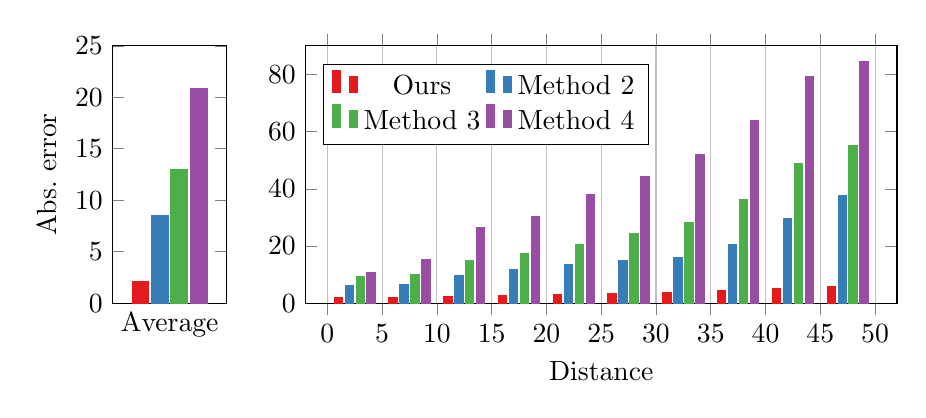
\begin{tikzpicture}
        \begin{groupplot}[
                bar cycle list/.style={
                        cycle list name=Set1,
                        every axis plot/.append style={fill, thin},
                    },
                enlarge x limits=0,
                group style={
                        group size=2 by 1,
                        horizontal sep=10mm,
                        xlabels at=edge bottom,
                        ylabels at=edge left,
                    },
                legend style={at={(0.03,0.93)}, anchor=north west,legend columns=2},
                ybar=1pt,
                ylabel={Abs.~error},
                ymin=0,
            ]
            \nextgroupplot[
                bar width=6pt,
                width=0.25\linewidth,
                symbolic x coords={Average},
                xlabel={Average},
                xmajorticks=false,
                ymax=0.25,
                ytick={0, 0.05, ..., 0.2501},
                yticklabels={0, 5, ..., 25},
            ]
            \addplot+ coordinates {(Average,0.0214)};
            \addplot+ coordinates {(Average,0.0851)};
            \addplot+ coordinates {(Average,0.1301)};
            \addplot+ coordinates {(Average,0.2088)};
            \nextgroupplot[
                bar width=3pt,
                width=0.75\linewidth,
                xlabel={Distance},
                xmajorgrids,
                xmax=52,
                xmin=-2,
                xtick={0, 5, ..., 50},
                ymax=0.9,
                ytick={0, 0.2, ..., 0.901},
                yticklabels={0, 20, ..., 90},
            ]
            \addplot+[bar shift=1] coordinates {(0,0.01863) (5,0.01864) (10,0.02215) (15,0.02521) (20,0.02945) (25,0.0342) (30,0.03805) (35,0.04333) (40,0.04947) (45,0.05766)};
            \addplot+[bar shift=2] coordinates {(0,0.06218) (5,0.06662) (10,0.09788) (15,0.11668) (20,0.1363) (25,0.15022) (30,0.15984) (35,0.20372) (40,0.2945) (45,0.37674)};
            \addplot+[bar shift=3] coordinates {(0,0.09407) (5,0.10072) (10,0.14832) (15,0.17394) (20,0.20679) (25,0.24182) (30,0.28272) (35,0.36184) (40,0.48994) (45,0.55175)};
            \addplot+[bar shift=4] coordinates {(0,0.10829) (5,0.15218) (10,0.26334) (15,0.30403) (20,0.3782) (25,0.44264) (30,0.52125) (35,0.63861) (40,0.79191) (45,0.84607)};
            \legend{Ours, Method 2, Method 3, Method 4}
        \end{groupplot}
    \end{tikzpicture}
    \caption{
        Abs.~errors of different models compared to ours.
        Left: Average errors. Right: Errors along distance.
    }
\end{figure}

\newpage
\section{Images}
\begin{figure}[h]
    \centering
    \begin{tikzpicture}
        \begin{axis}[
                axis equal image,
                axis on top,
                major grid style={very thin},
                enlargelimits=0,
                grid=major,
                height={},
                scale only axis=true,
                scaled x ticks=false,
                scaled y ticks=false,
                title=Reflections,
                title style={
                        anchor=north east,
                        at={(0.98,0.95)},
                        fill=white,
                    },
                xlabel={x},
                xmax=25,
                xmin=-25,
                xtick={-20, -10, ..., 20},
                ylabel={y},
                ymax=25,
                ymin=-25,
                ytick={-20, -10, ..., 20},
            ]
            \addplot graphics[xmin=-50,xmax=50,ymin=-50,ymax=50] {../res/sample.png};
            \addplot graphics[xmin=-2,xmax=2.8,ymin=-1.4,ymax=1.4] {../res/car.png};
        \end{axis}
    \end{tikzpicture}
    \caption{
        Reflections layer.
    }
\end{figure}

\end{document}